%\documentclass{nature}
\documentclass[12pt, letterpaper]{article}
\usepackage{graphicx}
%\usepackage{hyperref}
\usepackage{xcolor}
\usepackage[capposition=top]{floatrow}
\usepackage[center]{caption}
\usepackage{rotating}
\usepackage[flushleft]{threeparttable}
%\usepackage[superscript,biblabel]{cite}

%\bibliographystyle{naturemag}
%\usepackage{apacite}
\usepackage[style=nature]{biblatex}
%\usepackage[backend=biber,style=numeric,sorting=none]{biblatex}
%\usepackage[backend=biber]{biblatex}
\definecolor{green}{rgb}{0,1,0}
\newcommand{\NS}[1] {{\textcolor{green}{#1}}}
\newcommand{\TM}[1] {{\textcolor{orange}{#1}}}
\newcommand{\AT}[1] {{\textcolor{blue}{#1}}}

%I will need to fix the references
\addbibresource{football_refs.bib}
\begin{document}
\title{Reported cases of alcohol-related domestic abuse increase following the victory of the England national football team}
\author{Anna Trendl}
%title: I am using the word "reported" to highlight the issue of underreporting, and I am also cautious about not claiming causal effects, but emphasize that the increase starts when the match starts
\maketitle


%\textbf{Letter}:
%A Letter is an important research study of high quality and general interest to human behaviour researchers.  The text is approximately 5,000 words, including the introductory paragraph, but excluding references and figure legends. Letters should have no more than 4 display items (figures and/or tables). As a guideline, Letters contain approximately 30 references (excluding those cited exclusively in Methods). This format begins with a title of, at most, 90 characters (including spaces), followed by an introductory paragraph (not abstract) of approximately 200 words, summarizing the background, rationale, main results (introduced by "Here we show" or some equivalent phrase) and implications of the study. This paragraph should be fully referenced and should be considered part of the main text, so that any subsequent introductory material avoids too much redundancy with the introductory paragraph. Letters are not divided by headings, except for the Methods heading.
%
%Letters include received/accepted dates and may be accompanied by supplementary information. Letters are peer reviewed.
%
%\NS{Neil crappy abstract: When England wins or loses a football match, we use WMP data to show that there is a 60\% spike in domestic abuse cases.  We only see the patterns for wins and losses not draws, and only see the increase for domestic abuse cases involving alcohol. Indeed the spike is unique to male on female intimate partner domestic abuse, and we don't see it for other types of incident (e.g., antisocial behaviour).}

\section{Introductory para (200 words approx)}

Understanding the factors that contribute to the occurrence of violence in family and intimate partner relationships is key for designing effective interventions to protect victims. Previous research has suggested that national football (soccer) tournaments increase the number of reported domestic abuse cases in England\autocite{Kirby2014, Brimicombe2012}. While hypothesized to be a significant factor, previous quantitative research has not explored the role of alcohol in this relationship. Using crime data from the third largest police force in England, serving a population of 2.9 million\autocite{populationfigure}, we find that the number of reported alcohol-related domestic abuse cases increases by 61\% following an England victory in a national football tournament (World Cup, European Championship). This effect is specific to alcohol related incidents, with no detectable increase in non-alcohol related incidents. The effect is driven by an increase in male to female alcohol-related cases, and is absent from male to male, female to male, and female to female domestic abuse cases. We find similar patterns in other violent crimes. A three-hour analysis reveals that the increase starts in the three-hour period of the match, peaks in the three hours following the victory, and gradually declines to its baseline level in the 24 hours following the match. The abuse that occurs is not characteristically different from domestic abuse cases occurring on non-match days, apart from the stronger association with alcohol. 

\section{Long intro}

"If England gets beaten, so will she" - read the poster as part of the "The Not-So-Beautiful-Game" awareness campaign launched by the National Centre for Domestic Violence in the wake of the 2018 FIFA World Cup \autocite{NCDV}. While the link between sport events and domestic abuse has been the focus of a number of smaller studies\autocite{Williams2014}, large-scale quantitative investigations of this relationship are relatively scarce. The most extensive study in the topic found that an unexpected loss of the local National Football League (NFL) team resulted in a 10\% increase in the rate of reported male to female intimate partner violence (IPV) in the US\autocite{Card2011}. 

In England, most studies have focused on the link between football (soccer) and domestic abuse. Football's history is inextricably linked to England, and it is by far the most popular sport in the country \autocite{Parry2014}, with the 2018 World Cup attracting record number of viewers \autocite{BBC}. In 2012, a small, exploratory study investigated the effect of the 2010 World Cup on domestic abuse, using data from 33 out of 39 police forces in England\autocite{Brimicombe2012}. Using a control period from 2009, the study found that rates of reported domestic abuse increased significantly when England lost or won (about 33-35\%), but did not change on days when they drew. A more specific investigation, using daily counts of domestic abuse in Lancashire from the 2002, 2006 and 2010 World Cup, found a 38\% increase in the number of reported domestic violence cases when the England team lost, and a 26\% increase when they won or drew\autocite{Kirby2014}. These estimates had been widely discussed in the British media before the 2018 World Cup, and the figures were also quoted on the posters in the Not-so Beautiful Game Campaign. While domestic abuse is predominantly understood as a pattern of ongoing behaviour involving a series of occurrences, rather than a one-off incident triggered by football \autocite{Brooks-Hay2018}, these studies, and other qualitative investigations\autocite{Swallow} nevertheless suggest that national football tournaments can create an environment for abusers that is conducive to domestic abuse.

Why would national football tournaments, such as the World Cup or the European Championship precipitate domestic abuse? England's participation in these tournaments are times of heightened patriotic emotions and a strengthened sense of "Englishness", fuelled by media narratives that often use war references and a "us vs. them" rhetoric to generate and represent an English national identity\autocite{Vincent2014}. Previous qualtitatve research has suggested that televised contact sports can serve as vehicle for the male sports fan to redefine and express his masculinity in a way that allows dominance, control, and can ultimately manifest in the perpetration of domestic abuse, given susceptibility to such behaviours\autocite{Sabo,Swallow}. We speculate that this observation is especially pertinent in the context of England's participation in national tournaments, owing to the popularity of the sport in the country, the associated media attention, and the heightened sense of national consciousness.

Qualitative investigations suggest that alcohol can be a significant factor in the link between football and domestic abuse. Alcohol has a strong association with domestic abuse, those with alcohol-problems are more likely to be perpetrators, and when alcohol is involved, there is evidence that the violence might result in more serious injuries \autocite{Peralta2010}. However, it is generally understood that the role of alcohol should be considered in the context of a range of social, biological and pyschological factors, and that alcohol is never the direct cause of domestic abuse \autocite{Javaid2015,Peralta2010}. One explanation for the co-occurrence of domestic abuse and alcohol suggest that for some men, drinking and violence plays an instrumental role in the construction and expression of masculinity, especially when the problem of masculine deficiency is present (e.g., by unemployment)\autocite{Peralta2010}. 

In the US, the relationship between unexpected NFL losses and IPV did not depend on alcohol-involvement in the incident\autocite{Card2011}. While England-based quantitative studies did not look at the role of alcohol in particular. Given the strong association between drinking culture and football in England\autocite{Dixon2014}, a relationship continuously reinforced by the marketing practices of the alcohol industry\autocite{Gornall2014}, we hypothesize that alcohol play an important role in the relationship between national football tournaments and domestic abuse.

To explore this hypothesis, we investigate whether the number of reported domestic abuse cases recorded by the West Midland Police in England between 2010 and 2018 increase on days when the England national team plays in the World Cup or the European Championship, and whether the effect, if any, is affected by alcohol-involvement in the reported case. We also consider whether the result of the match alters the relationship, as previous research suggested that the effect is heightened when England loses\autocite{Kirby2014}. Our unique dataset further allows us to investigate various aspects of the link between football tournaments and domestic abuse.


\newpage

\subsection{Data description}

Our dataset comprises all crimes and specific types of incidents (such as domestic abuse) that have been reported to the West Midlands Police (the third largest police force in England\autocite{Homeoffice}, serving an estimated 2.9 million people in 2017\autocite{populationfigure}) in the period between 2010 and 2018\footnote{The first half of 2017 has been excluded due to missing data.}. The number of reported domestic abuse cases is the sum of crimes that have a domestic abuse marker, and all domestic abuse incidents. Crimes that have a domestic abuse marker indicate cases of domestic abuse that meet the criteria for notifiable offences in the UK, whereas domestic abuse incidents refer to cases that do not qualify as a crime. For each record in this dataset, we have information about the time and location of the incident or crime, and the gender and age of the offender and victim. We can also identify repeat offenders and victims by their unique person identifier. Domestic abuse cases comprise about 31\% of all recorded crimes and incidents in the dataset, and about 23\% of all domestic abuse cases are alcohol-related. \textcolor{red}{Sentence about daily rate and how it compares to previous studies}. There were three World Cups (2010, 2014, 2018) and two European Championships (2012, 2016) in the period covered by our dataset. All included tournaments took place in the months of June and July.

In the UK, the term "domestic abuse" refers to a wide range of behaviours, from physical and sexual violence to psychological, emotional, financial abuse, threatening behaviour, stalking and harassment either within a family or an intimate relationship\autocite{ONS}. Recent changes to the definition introduced the concept of coercive control, which recognises domestic abuse as a pattern of incidents, which can include any of the above behaviours. Previous research has mostly focused on IPV, which the largest subcategory of domestic abuse. 


\begin{table}[ht]
\centering
\caption{\textcolor{red}{this table is just for illustration}}
\begin{tabular}{rrlrrrr}
  \hline
 & year & Alcohol & No\_days & DA\_cases & Population & Rate \\ 
  \hline
1 & 2010 & No & 365 & 23332.00 & 2711938.00 & 2.36 \\ 
  2 & 2010 & Yes & 365 & 3978.00 & 2711938.00 & 0.40 \\ 
  3 & 2011 & No & 365 & 20887.00 & 2739733.00 & 2.09 \\ 
  4 & 2011 & Yes & 365 & 3490.00 & 2739733.00 & 0.35 \\ 
  5 & 2012 & No & 366 & 15789.00 & 2761887.00 & 1.56 \\ 
  6 & 2012 & Yes & 366 & 3611.00 & 2761887.00 & 0.36 \\ 
  7 & 2013 & No & 365 & 22422.00 & 2781753.00 & 2.21 \\ 
  8 & 2013 & Yes & 365 & 7732.00 & 2781753.00 & 0.76 \\ 
  9 & 2014 & No & 365 & 27758.00 & 2805891.00 & 2.71 \\ 
  10 & 2014 & Yes & 365 & 10005.00 & 2805891.00 & 0.98 \\ 
  11 & 2015 & No & 365 & 30225.00 & 2834490.00 & 2.92 \\ 
  12 & 2015 & Yes & 365 & 10931.00 & 2834490.00 & 1.06 \\ 
  13 & 2016 & No & 366 & 31499.00 & 2870551.00 & 3.00 \\ 
  14 & 2016 & Yes & 366 & 11005.00 & 2870551.00 & 1.05 \\ 
  15 & 2017 & No & 365 & 12909.00 & 2897303.00 & 1.22 \\ 
  16 & 2017 & Yes & 365 & 4232.00 & 2897303.00 & 0.40 \\ 
  17 & 2018 & No & 310 & 28479.00 &  &  \\ 
  18 & 2018 & Yes & 310 & 9109.00 &  &  \\ 
   \hline
\end{tabular}
\end{table}

Our dataset contains all cases of domestic abuse that have been reported to the police, but the vast majority of all domestic abuse incidents in fact never get reported (according to the Crime Survey of England and Wales, only 17\% of all domestic abuse victims reported the abuse to the police between April, 2017 and March, 2018\autocite{ONS}). This substantial reporting bias, and its potential correlation with other contextual factors warrants a careful interpretation of the estimates from any quantitative study investigating domestic abuse, and highlights the importance of utilising a mixed methods approach to explore the factors facilitating domestic abuse. 

\textcolor{red}{Card \& Dahl find a 10\% increase in male to female violence, in their dataset, daily prevalence of DA is 1.28 per 100,000 population, 10\% increase is 0.128 increase in daily rate, but the average is 0.70 (excluding 2017 and 2018), 60\% increase is 0.42 increase in daily rate}

\clearpage


\section{Results}

In the following regressions, each observation is a day in the period between 2010 and 2018, and the outcome variable is the number of domestic abuse cases reported to have been perpetrated on that day. To investigate whether national football tournaments affect the number of reported abuse cases, we classify each day in our dataset as either a day on which England won (England win), lost (England lost) or drew (England draw), a day after an England match day (After England), any other day during the tournament (Tournament on), or any other day during the rest of the year (Nonmatch day). 

Using a series of negative binomial regressions, we first compare various, increasingly complex model specifications to understand the relationship between football, alcohol and domestic abuse. Adding type of day as an explanatory variable to a model with only alcohol and time controls marginally improves the model fit (see column 2 in Table \ref{specifications}), and the results show a 20\%, 95\% CI [5--38] increase in the number of reported domestic abuse cases when the England national football team wins. The comparison between column 2 and 3 reveals that this increase stems from a much more pronounced, 61\%, 95\% CI [24--110] increase within the subgroup of alcohol-related domestic abuse cases on days when England wins. \TM{Should we comment on the lack of effect for draws and losses?}

Further interacting alcohol with the rest of the time-specific control variables results in a substantially improved model fit (see column 4), but does not alter the effect of an England win on alcohol-related domestic abuse (61\%, 95\% CI [32--96]). The results also reveal a smaller, 9\%, 95\% CI [1-17] increase on days following an England match day, potentially the result of a temporal spillover effect of the match, and an 8\%, 95\% CI [2-14] decrease in alcohol-related incidents during tournament days that are not England match days, or days after an England match days. \AT{I find this a bit puzzling} \TM{People do all their drinking on days when the matches are on, and are then hungover/working the other days? Repeat perpetrators still being in a cell the next day? I don't think we necessarily need to provide an explanation}



\begin{table*}
\centering
\scalebox{0.9}{
  \begin{threeparttable}
  \caption{Number of reported domestic abuse incidents by alcohol involvement and type of day} 
  \label{specifications}
\begin{tabular}{@{\extracolsep{5pt}}lcccc} 
\\[-1.8ex]\hline 
\hline \\[-1.8ex] 
 & \multicolumn{4}{c}{\textit{Dependent variable:}} \\ 
\cline{2-5} 
\\[-1.8ex] & \multicolumn{4}{c}{Number of reported domestic abuse cases per day} \\ 
\\[-1.8ex] & (1) & (2) & (3) & (4)\\ 
\hline \\[-1.8ex] 
Alcohol & $-$0.719$^{***}$ & $-$0.719$^{***}$ & $-$0.719$^{***}$ & $-$0.862$^{***}$ \\ 
  & (0.007) & (0.007) & (0.008) & (0.031) \\ 
  Tournament on &  & $-$0.004 & 0.014 & 0.032 \\ 
  &  & (0.023) & (0.027) & (0.020) \\ 
  England win &  & 0.205$^{***}$ & $-$0.037 & $-$0.031 \\ 
  &  & (0.069) & (0.091) & (0.063) \\ 
  England draw &  & 0.025 & 0.048 & 0.047 \\ 
  &  & (0.082) & (0.104) & (0.072) \\ 
  England lost &  & 0.078 & $-$0.013 & 0.050 \\ 
  &  & (0.068) & (0.089) & (0.061) \\ 
  After England &  & 0.097$^{**}$ & 0.075 & 0.086$^{**}$ \\ 
  &  & (0.043) & (0.055) & (0.038) \\ 
  Tournament on:Alcohol &  &  & $-$0.043 & $-$0.083$^{**}$ \\ 
  &  &  & (0.040) & (0.035) \\ 
  England win:Alcohol &  &  & 0.610$^{***}$ & 0.606$^{***}$ \\ 
  &  &  & (0.135) & (0.101) \\ 
  England draw:Alcohol &  &  & $-$0.055 & $-$0.034 \\ 
  &  &  & (0.165) & (0.129) \\ 
  England lost:Alcohol &  &  & 0.223 & 0.076 \\ 
  &  &  & (0.135) & (0.101) \\ 
  After England:Alcohol &  &  & 0.051 & 0.037 \\ 
  &  &  & (0.084) & (0.066) \\ 
 \hline \\[-1.8ex] 
Observations & 6,034 & 6,034 & 6,034 & 6,034 \\ 
AIC & 45,539.500 & 45,536.770 & 45,530.360 & 41,959.280 \\ 
%BIC & 45740.656 & 45771.447 & 45798.563 & 42408.524 \\ 
\hline 
\hline \\[-1.8ex] 
%\textit{Note:}  & \multicolumn{4}{r}{$^{*}$p$<$0.1; $^{**}$p$<$0.05; $^{***}$p$<$0.01} \\ 
\end{tabular} 
\begin{tablenotes}
      \item[a] \textit{$^{*}$p$<$0.1; $^{**}$p$<$0.05; $^{***}$p$<$0.01}
      \item[b] \textit{Estimates are from a series of negative binomial regressions (based on tests of overdispersion)  with year, month, day of week, Christmas, New Year's eve controls; Model 4 further includes interactions between alcohol and all control variables; standard errors in parentheses}
    \end{tablenotes}
\end{threeparttable} }
\end{table*}

To explore where this increase comes from, we investigate whether the effect is sensitive to the gender of the perpetrator and the victim. Previous qualitative research has suggested that the link between football and domestic abuse is a result of violent expression of masculinity, where heavy drinking is also often present\autocite{Sabo}. If this was the case, we would expect football and alcohol to only affect reported numbers of male-perpetrated domestic abuse. 


The first column of Table \ref{gender_regression} shows the result for different offender-victim gender groups. The results show that the effect is only present in the subgroup of Male to Female abuse (which comprises about 80\% of all domestic abuse cases in our data), where the increase is 67\%, 95\% CI [35--107]. These results can be viewed in light of the observation that British football fandom is prevalently male-dominated \autocite{Parry2014}, and they lend support to the hypothesis that masculinity construction and alcohol may be key to the link between football and domestic abuse.

\begin{table}
\centering
\scalebox{0.85}{
  \begin{threeparttable}
  \caption{Number of reported domestic abuse incidents by type of day, alcohol involvement, and gender of perpetrator and victim} 
  \label{gender_regression}
\begin{tabular}{@{\extracolsep{5pt}}lcccc} 
\\[-1.8ex]\hline 
\hline \\[-1.8ex] 
 & \multicolumn{4}{c}{\textit{Dependent variable:}} \\ 
\cline{2-5} 
\\[-1.8ex] & \multicolumn{4}{c}{Number of reported domestic abuse cases per day} \\ 
\\
 & Male & Male & Female & Female \\ 
 & to Male & to Female & to Female & to Male \\ 
\\[-1.8ex] & (1) & (2) & (3) & (4)\\ 
\hline \\[-1.8ex] 
%Alcohol & $-$0.825$^{***}$ & $-$0.870$^{***}$ & $-$0.808$^{***}$ & $-$0.858$^{***}$ \\ 
%  & (0.101) & (0.034) & (0.133) & (0.080) \\ 
  Tournament on & 0.005 & 0.038$^{*}$ & 0.053 & $-$0.048 \\ 
  & (0.054) & (0.021) & (0.062) & (0.045) \\ 
  England win & $-$0.068 & $-$0.022 & 0.019 & $-$0.147 \\ 
  & (0.165) & (0.066) & (0.193) & (0.135) \\ 
  England draw & 0.080 & 0.038 & 0.043 & 0.107 \\ 
  & (0.194) & (0.076) & (0.225) & (0.169) \\ 
  England lost & $-$0.063 & 0.065 & $-$0.036 & 0.117 \\ 
  & (0.162) & (0.064) & (0.171) & (0.136) \\ 
  After England & $-$0.036 & 0.093$^{**}$ & 0.152$^{*}$ & 0.025 \\ 
  & (0.103) & (0.040) & (0.114) & (0.082) \\ 
  Alcohol:Tournament on & $-$0.181$^{*}$ & $-$0.077$^{**}$ & $-$0.018 & $-$0.215$^{*}$ \\ 
  & (0.106) & (0.038) & (0.137) & (0.084) \\ 
  Alcohol:England win & 0.334 & 0.674$^{***}$ & 0.360 & 0.472 \\ 
  & (0.285) & (0.108) & (0.358) & (0.231) \\ 
  Alcohol:England draw & $-$0.282 & 0.031 & 0.071 & $-$0.580 \\ 
  & (0.411) & (0.138) & (0.629) & (0.313) \\ 
  Alcohol:England lost & 0.286 & 0.028 & 0.328 & $-$0.088 \\ 
  & (0.279) & (0.111) & (0.356) & (0.231) \\ 
  Alcohol:After England & 0.209 & 0.052 & $-$0.111 & $-$0.040 \\ 
  & (0.185) & (0.071) & (0.242) & (0.159) \\ 
 \hline \\[-1.8ex] 
Observations & 6,034 & 6,034 & 6,034 & 6,034 \\ 
%Log Likelihood & $-$10,637.300 & $-$19,923.970 & $-$9,234.791 & $-$12,372.460 \\ 
%$\theta$ & 141.533  (111.012) & 59.918$^{***}$  (2.924) & 64.457$^{**}$  (31.740) & 60.289$^{***}$  (14.059) \\ 
%Akaike Inf. Crit. & 21,406.600 & 39,979.950 & 18,601.580 & 24,876.910 \\ 
%\hline 
\hline \\[-1.8ex] 
%\textit{Note:}  & \multicolumn{4}{r}{$^{*}$p$<$0.1; $^{**}$p$<$0.05; $^{***}$p$<$0.01} \\ 
\end{tabular} 
\begin{tablenotes}
      \item[a] \textit{$^{*}$p$<$0.1; $^{**}$p$<$0.05; $^{***}$p$<$0.01}
      \item[b] \textit{Estimates are from a series of negative binomial regressions (based on tests of overdispersion)  with year, month, day of week, Christmas, New Year's eve controls interacted with alcohol; standard errors in parentheses}
    \end{tablenotes}
\end{threeparttable} }
\end{table}


Our unique dataset further allows us to explore whether England games have similar effects on other types of criminal behaviours. Specifically, we are interested in how an England match day affects the number of reported property-related crimes (including burglary, theft and robbery), public order offences (behaviours that cause offence to the general public), hate crimes (hate incidents and any other racially or religiously aggravated crime), and other violent crimes (excluding cases of domestic abuse). Of particular interest is the effect of football on non-domestic violent crimes, since it is possible that alcohol-fuelled violence that follows an England victory is not limited to family relationships.

Table \ref{othertype_regression} shows the results from a series of negative binomial regression for different types of criminal behaviours. These reveal that while property-related offences are not affected by football, there is an increase in the number of non-alcohol related public order offence cases on tournament days, when England wins, and on days after and England game. Hate incidents with no alcohol involvement also increase when the tournament is on. But most importantly, we find a similar pattern for other violent crimes, namely, a 55\%, 95\% [43--72] increase in alcohol-related violent offences when England wins, and a smaller increase on days following an England match. This result highlights that football-induced and alcohol-related violent behaviour is not limited to family relationships. Further analysis reveals that the increase in these alcohol-related non-domestic violent crimes also predominantly comes from Male to Female cases (although Male to Male and Female to Male cases also contribute, see Table \ref{othertype_regression} in the Appendix). These results strongly suggest that football and alcohol only make men more violent and mostly towards women. \AT{Is this too harsh? I added this analysis because I think it strengthens our point about how football makes men more violent. Also I wonder why they would beat up women they don't know - can be a result of the noisiness of the DA indicator?} \TM{I think this is very good}




\begin{table}[!htbp]
 \centering 
 \scalebox{0.8}{
  \begin{threeparttable}
  \caption{Number of reported cases for each crime type, by type of day, and alcohol involvement} 
  \label{othertype_regression}
\begin{tabular}{@{\extracolsep{5pt}}lcccc} 
\\[-1.8ex]\hline 
\hline \\[-1.8ex] 
 & \multicolumn{4}{c}{\textit{Dependent variable:}} \\ 
 \\[-1.8ex] & \multicolumn{4}{c}{Number of reported domestic abuse cases per day} \\ 
\cline{2-5} 
 & Property- & Public Order & Hate & Other \\ 
  & related &  Offences & incidents & violence \\ 
\\[-1.8ex] & (1) & (2) & (3) & (4)\\ 
\hline \\[-1.8ex] 
% Alcohol & $-$0.981$^{***}$ & $-$0.922$^{***}$ & $-$0.934$^{***}$ & $-$0.902$^{***}$ \\ 
%  & (0.065) & (0.080) & (0.115) & (0.040) \\ 
  Tournament on & 0.042 & 0.096$^{**}$ & 0.138$^{***}$ & 0.034 \\ 
  & (0.026) & (0.036) & (0.047) & (0.027) \\ 
  England win & 0.052 & 0.234$^{**}$ & 0.073 & 0.094 \\ 
  & (0.074) & (0.095) & (0.136) & (0.077) \\ 
  England draw & 0.100 & $-$0.065 & $-$0.066 & 0.035 \\ 
  & (0.085) & (0.128) & (0.168) & (0.092) \\ 
  England lost & $-$0.042 & 0.075 & 0.011 & 0.089 \\ 
  & (0.078) & (0.100) & (0.139) & (0.078) \\ 
  After England & 0.052 & 0.161$^{**}$ & 0.141 & 0.108$^{**}$ \\ 
  & (0.047) & (0.062) & (0.084) & (0.048) \\ 
  Alcohol:Tournament on & 0.135 & $-$0.197$^{**}$ & $-$0.215$^{*}$ & $-$0.009 \\ 
  & (0.080) & (0.101) & (0.141) & (0.051) \\ 
  Alcohol:England win & 0.259 & 0.020 & 0.310 & 0.507$^{***}$ \\ 
  & (0.219) & (0.256) & (0.359) & (0.132) \\ 
  Alcohol:England draw & 0.060 & 0.374 & 0.393 & 0.360$^{*}$ \\ 
  & (0.264) & (0.303) & (0.431) & (0.161) \\ 
  Alcohol:England lost & 0.144 & 0.456$^{*}$ & $-$0.032 & 0.018 \\ 
  & (0.226) & (0.228) & (0.393) & (0.138) \\ 
  Alcohol:After England & 0.094 & 0.127 & 0.446$^{*}$ & 0.053 \\ 
  & (0.144) & (0.158) & (0.211) & (0.088) \\ 
 \hline \\[-1.8ex] 
Observations & 6,034 & 6,034 & 6,034 & 6,034 \\ 
%Log Likelihood & $-$16,843.670 & $-$13,757.560 & $-$11,391.050 & $-$20,108.820 \\ 
%$\theta$ & 40.698$^{***}$  (1.891) & 33.673$^{***}$  (2.784) & 24.170$^{***}$  (2.563) & 30.562$^{***}$  (1.167) \\ 
%Akaike Inf. Crit. & 33,819.350 & 27,647.120 & 22,914.090 & 40,349.640 \\ 
\hline 
\hline \\[-1.8ex] 
%\textit{Note:}  & \multicolumn{4}{r}{$^{*}$p$<$0.1; $^{**}$p$<$0.05; $^{***}$p$<$0.01} \\ 
\end{tabular} 
\begin{tablenotes}
      \item[a] \textit{$^{*}$p$<$0.1; $^{**}$p$<$0.05; $^{***}$p$<$0.01}
      \item[b] \textit{Estimates are from a series of negative binomial regressions (based on tests of overdispersion)  with year, month, day of week, Christmas, New Year's eve controls interacted by alcohol; standard errors in parentheses}
    \end{tablenotes}
\end{threeparttable} }
\end{table}


Next, we explore the temporal dynamics of the increase in alcohol-related domestic abuse on England match days in more detail. To this end, we divided each day in our dataset into eight three-hour periods, the first one starting at 12am, and used these to identify specific time windows around the time of the match. The exact time of the matches vary considerably (the earliest starting at 1pm, and the latest at 11pm). We first identified the three-hour period of the day into which each match falls. If the start and end time of the match did not fall in the same three-hour period, we chose the three-hour period that covers the larger part of the match (e.g., a 2.5 hour long match starting at 7pm will be assigned to the 6-9pm period and not to the 9pm-12am period). Based on our previous results, we analyse the effect by the result of the match and alcohol-involvement in the case, by running two separate regressions for alcohol and non-alcohol related domestic abuse cases.

Figure \ref{fig:threehours} shows a plot of the coefficients from these negative binomial regressions, revealing a stark increase in alcohol-related domestic abuse on days of an England victory, starting in the three hour period of the match, peaking in the three-hour period afterwards, and gradually declining to its original level in the twenty-four hours following the victory. These results strongly suggest that the emotional effect of a win drive the subsequent increase in alcohol-related domestic abuse and highlight the possibility that the effect of England victories might stem from prolonged post-match celebrations coupled with increased alcohol consumption.  Interestingly, we also see a slight increase in non-alcohol related incidents twelve hours after a loss or a victory, probably reflecting the small increase in non-alcohol related domestic abuse after an England match day seen in Table \ref{specifications}.


\begin{figure}
\centering
 \caption{The temporal dynamics of the effect}
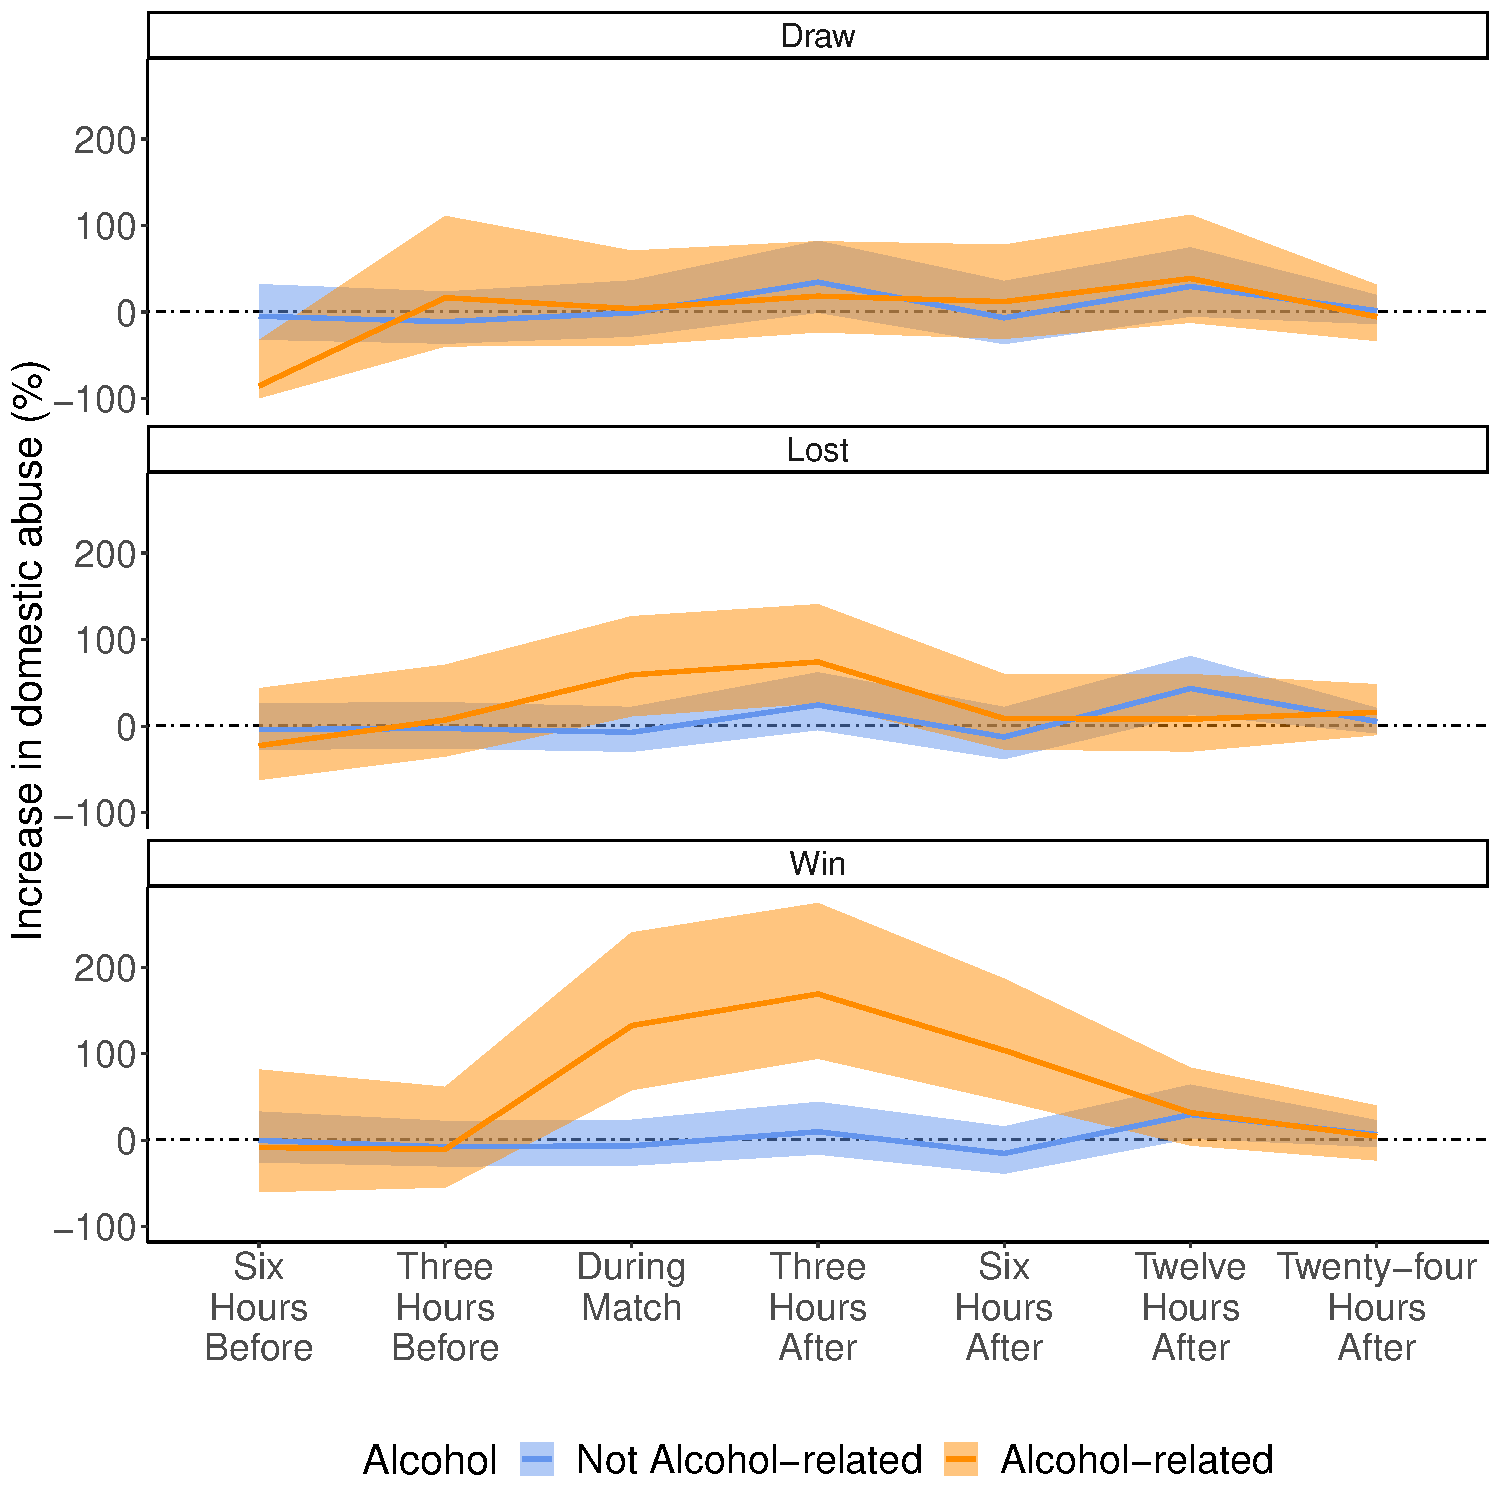
\includegraphics[width=0.75\textwidth]{Threehours.pdf}
\label{fig:threehours}
\floatfoot{Note: Estimates are from two separate negative binomial regressions (based on tests of overdispersion) with year, month, day of week, three-hour period of day, Christmas, New Year's eve controls}
\end{figure}

\newpage

\section{Discussion}

While only 23\% of all domestic abuse cases are alcohol-related in our dataset, the estimated effect of a 60\% increase in alcohol-related domestic abuse cases is large, translating into a 0.42 increase in the daily rate of \textit{reported} alcohol-related domestic abuse cases per 100,000 individuals. Our results constitute the first quantitative evidence that alcohol plays an instrumental role in the relationship between football and domestic abuse in England, and that the effect is exclusively limited to male-perpetrated domestic abuse. The effect is about 70\% of a Christmas effect on alcohol-related domestic abuse. \AT{OR This estimate is comparable to a 89\% increase in alcohol-related domestic abuse cases at Christmas?.} \TM{I don't think most people would associate Christmas with huge increases in DA. I think this summary is already really strong without this comparison}
 

Our findings show both similarities and differences with results from previous quantitative investigations. Similarly to a previous study, we found that it is male to female abuse that is affected by a sporting event\autocite{Card2011}. However, in the same study, the effect of the match did not depend on alcohol-involvement in the abuse case, and the increase was driven by unexpected losses, whereas our findings suggest that it is a victory that results in the largest increase, and that alcohol plays an instrumental role in the relationship between football and domestic abuse. This discrepancy most likely stems from the contextual differences between the two studies (England, football, national tournaments vs. US, American football, NFL matches), highlighting that the effect on sports-induced emotional cues on domestic abuse are sensitive to the cultural context. 

Based on the pre-match betting odds, all England victories were expected in our dataset, suggesting that in the context of England's participation in national football tournaments, it is living up to the hopes of the fans that has the largest emotional effect, and perhaps results in increased alcohol consumption\autocite{Davies2018}. Indeed, English newspapers' narratives about the team's performance in these tournaments are characterised with high levels of optimism, expectation and yearning for the glory of the 1966 World Cup\autocite{Vincent2010}. Previous research has demonstrated how the vicarious experience of watching their team play can increase supporter's testosterone and cortisol levels, even when they expect their team to win, suggested to be an adaptive response to the perceived threat to one's social identity\autocite{VanderMeij2012}.

%In the context of the World Cup, previous research has reported elevated testosterone levels amongst the winning team's supporters\autocite{Bernhardt1998}.

The largest England-based study found that an England loss results in the largest increase (38\%) in domestic abuse, and a win or draw have a slightly smaller effect (26\%)\autocite{Kirby2014}. We find a markedly different pattern, in that it is when England wins we find a substantial increase in alcohol-related domestic abuse, whereas we found no comparable effects for an England loss. Upon re-analysing their data by treating wins and draws as two separate variables (resulting in an improved model fit, see Table \ref{kirbyrep1} in the Appendix), we see a roughly similar effect for wins (45\%, 95\% CI [28--64]) and losses (39\%, 95\% CI [18--64]), and no effect when England draws (probably due to the fact that high-stake matches after the group-stage in the tournament cannot result in a draw). A stark difference between our results is the lack of an England loss effect in our sample. While our study is different in a few aspects (West Midlands 2010-2018 vs Lancashire, 2002, 2006, 2010), the discrepancy is still puzzling given that these are \textit{national} football tournament matches.

To explore the underlying reason for this discrepancy and test the robustness of our results, we find it instructive to analyse the the patterns by specific tournament years for the two datasets (see Table \ref{kirbyrep2} in the Appendix). An interesting common pattern in both datasets is the large effect of England's victory over Slovenia in the group stage of the 2010 World Cup, which, after much anticipation, secured their progression to the next stage of the tournament. Equally, the subsequent loss against Germany in the knockout stage resulted in a substantial increase in the number of reported domestic abuse incidents, which is the only tournament in our dataset where this pattern appears. While the effect of a victory or loss is likely to be highly specific to the context of a particular match (e.g., group stage or knockout stage, previous performance of the team, weather on the day, etc.), the estimated effect of an England victory on the number of reported domestic abuse cases is robust to different model specifications (see Table \ref{specifications}),  using data from a different geographical area (see Table \ref{kirbyrep2} in the Appendix), and the exclusion of specific tournament years (see Table \ref{robustness} in the Appendix). \TM{Do we also want to emphasize the differnce in sample size, and representativeness between west mids and Lancashire?}


Does this effect generalise to other sporting events, or is it specific to football?
It has been suggested previously that popular sports, such as rugby have similar links with domestic abuse\autocite{Brooks-Hay2018}. Focusing on the Six Nations, a high-profile rugby tournament that takes place every year with the participation of England, Wales, Scotland, Ireland, France and Italy, we explored whether the reported number of domestic abuse cases increase on days when the England national rugby team plays. Since the Six Nations takes place every year with 15 matches for each team as opposed to the World Cup and the European Championship, which are relatively rare, we have many more days when England lost or won. The results show no comparable effects for rugby matches (see Table \ref{rugby} in the Appendix), which might stem from differences in media coverage and audience numbers between the two tournaments.  \TM{Is it worth including a citation that Rugby is the second most watched sport after football? American reviewers may never have heard of it and assume it is too niche}

We also investigated whether similar patterns are also present in other types of crimes, which are similar to domestic abuse in nature. Specifically, we explored how England's participation in national football tournaments affects alcohol and non-alcohol related reported sexual offences and other types of abuse (child abuse, vulnerable adult abuse). The results show no effect on the number of reported sexual offences, and a slight increase in the number of reported other cases when the tournament is on (see Table \ref{otherabuse} in the Appendix). 

Our data allows us to explore the characteristics of alcohol-related domestic abuse cases reported on England match days. First, using a series of logistic regressions, we investigate whether these cases are more likely to be newly reported (in the sense that there was no earlier reported case with the same victim and offender in our dataset), happen inside (in a residential dwelling) as opposed to a public location, or result in an injury. We find no evidence that cases reported on England match days are more likely to be newly reported cases (see Table \ref{Characteristics1} in the Appendix). It could be argued that on England match days, cases of domestic abuse are more likely to happen outside and subsequently get reported compared to non-match days, due to the large number of fans congregating in pubs. Interestingly, reported cases are more likely to happen in public on England lost days but not on England win days, and this effect does not differ by alcohol-involvement in the case. Non-alcohol related cases reported on England lost days are also more likely to result in injury, a pattern that is absent in alcohol-related cases.

Next we turn to repeated cases (multiple cases with the same victim-offender pair). We are interested in whether the number of days elapsed between two consecutive cases is affected by England football matches. For example, it is possible that England match days bring reported cases of domestic abuse forward, which would have otherwise happened at a later point in time. To investigate this question, we run two negative binomial regressions, where the outcome variable is the number of days elapsed since the last reported case and the number of days until the next case. 

The results show that non-alcohol related cases perpetrated on England loss days are slightly more likely to occur sooner after the previous incident, compared to repeat cases happening on non-match days, but only for non-alcohol related incidents (see Table \ref{Characteristics2} in the Appendix). Non-alcohol related domestic abuse cases perpetrated on England win days are more likely to be followed by another case of abuse sooner, compared to cases occurring on non-match days, and this pattern is absent from alcohol-related cases. Interestingly, non-alcohol related cases perpetrated on England match days or after and England match, and alcohol-related cases on an England draw day are more likely to be reported sooner. \TM{I think this is a really interesting result! Potentially a nice link back to the Card and Lee results.}

Finally, we are interested in whether an England match day transforms previously non-alcohol related incidents into alcohol-related ones. To explore this question, we ran a logistic regression on the subset of repeated cases, controlling for the type of the previous case (alcohol/non-alcohol related). We find that an England win day increases the likelihood of an alcohol-related case occurring, irrespective of whether the previous case was alcohol-related or not (see Table \ref{alctrans} in the Appendix).

\AT{These results are weird...}

These results indicate that apart from the higher likelihood of alcohol-involvement, domestic abuse cases perpetrated on England win days are not characteristically different from domestic abuse cases perpetrated on other days during the year. However, the high level of underreporting of domestic abuse cases warrant a cautious interpretation of these findings. 

 Nevertheless, taken together, our results suggest that the increase is unlikely to be a result of changes in the victim's willingness to report cases (e.g., due to awareness campaigns). Other suggested explanations for the observed increase in the number of reported cases of domestic abuse on England match days include other high-profile events taking place around the time of the match and increased policing on the day \autocite{Brooks-Hay2018}. Our three-hour analysis of the England win effect (Figure \ref{fig:threehours}) show that the temporal pattern of the effect is highly consistent with a match-induced explanation of the increase. In addition, it is unclear why the effect of different policing practices would depend on the result of the match. 


\subsection{Limitations}



\newpage

\section*{Appendix}

\begin{table}[ht]
\centering
 \caption{Non-domestic violent cases by gender}
  \label{otherviolence_gender}
 \scalebox{0.9}{
   \begin{threeparttable}
\begin{tabular}{@{\extracolsep{5pt}}lcccc} 
\\[-1.8ex]\hline 
\hline \\[-1.8ex] 
 & \multicolumn{4}{c}{\textit{Dependent variable:}} \\ 
\cline{2-5} 
\\[-1.8ex] & \multicolumn{4}{c}{Number of other violent abuse cases per day} \\ 
\\
 & Male & Male & Female & Female \\ 
 & to Male & to Female & to Female & to Male \\ 
\\[-1.8ex] & (1) & (2) & (3) & (4)\\ 
\hline \\[-1.8ex] 
% Alcohol & $-$0.900$^{***}$ & $-$0.891$^{***}$ & $-$0.864$^{***}$ & $-$0.921$^{***}$ \\ 
%  & (0.048) & (0.033) & (0.080) & (0.066) \\ 
  Tournament on & 0.037 & 0.050$^{**}$ & 0.041 & 0.051 \\ 
  & (0.026) & (0.021) & (0.038) & (0.036) \\ 
  England win & 0.013 & 0.019 & $-$0.031 & 0.174 \\ 
  & (0.082) & (0.067) & (0.111) & (0.112) \\ 
  England draw & 0.089 & 0.012 & 0.115 & 0.042 \\ 
  & (0.094) & (0.078) & (0.139) & (0.132) \\ 
  England lost & 0.018 & 0.028 & 0.088 & 0.118 \\ 
  & (0.082) & (0.066) & (0.114) & (0.108) \\ 
  After England & 0.085 & 0.070 & 0.181$^{**}$ & 0.149$^{**}$ \\ 
  & (0.050) & (0.042) & (0.071) & (0.067) \\ 
  Alcohol:Tournament on & $-$0.027 & $-$0.086$^{**}$ & $-$0.077 & $-$0.167$^{**}$ \\ 
  & (0.055) & (0.038) & (0.087) & (0.073) \\ 
  Alcohol:England win & 0.391$^{**}$ & 0.613$^{***}$ & 0.441$^{*}$ & $-$0.114 \\ 
  & (0.158) & (0.109) & (0.251) & (0.199) \\ 
  Alcohol:England draw & 0.071 & 0.102 & 0.127 & $-$0.337 \\ 
  & (0.192) & (0.137) & (0.361) & (0.254) \\ 
  Alcohol:England lost & 0.296$^{*}$ & 0.057 & $-$0.023 & 0.027 \\ 
  & (0.153) & (0.112) & (0.237) & (0.207) \\ 
  Alcohol:After England & 0.208$^{*}$ & 0.053 & $-$0.119 & $-$0.158 \\ 
  & (0.100) & (0.072) & (0.163) & (0.136) \\ 
 \hline \\[-1.8ex] 
Observations & 6,034 & 6,034 & 6,034 & 6,034 \\ 
%Log Likelihood & $-$17,204.240 & $-$21,360.820 & $-$13,708.300 & $-$14,378.320 \\ 
%$\theta$ & 44.231$^{***}$  (2.800) & 43.449$^{***}$  (1.546) & 24.998$^{***}$  (1.919) & 35.978$^{***}$  (3.376) \\ 
%Akaike Inf. Crit. & 34,540.480 & 42,853.640 & 27,548.590 & 28,888.630 \\ 
\hline 
\hline \\[-1.8ex] 
%\textit{Note:}  & \multicolumn{4}{r}{$^{*}$p$<$0.1; $^{**}$p$<$0.05; $^{***}$p$<$0.01} \\ 
\end{tabular} 
\begin{tablenotes}
     \item[a] \textit{$^{*}$p$<$0.1; $^{**}$p$<$0.05; $^{***}$p$<$0.01}
      \item[b] \textit{Estimates are from a series of negative binomial regressions (based on tests of overdispersion)  with year, month, day of week, Christmas, New Year's eve controls interacted with alcohol; standard errors in parentheses}
    \end{tablenotes}
\end{threeparttable} }
\end{table}

\newpage

\begin{table}
\centering
 \caption{Replication of Kirby et al. (2014) with an alternative specification}
   \label{kirbyrep1}
 \begin{threeparttable}
\begin{tabular}{@{\extracolsep{5pt}}lcc} 
\\[-1.8ex]\hline 
\hline \\[-1.8ex] 
 & \multicolumn{2}{c}{\textit{Dependent variable:}} \\ 
\cline{2-3} 
\\[-1.8ex] & \multicolumn{2}{c}{Number of reported IPV cases per day} \\ 
\\ 
 & Original Model & Win/Draw Separate \\ 
\\[-1.8ex] & (1) & (2)\\ 
\hline \\[-1.8ex] 
 England windraw & 0.256$^{***}$ &  \\ 
  & (0.055) &  \\ 
  England win &  & 0.452$^{***}$ \\ 
  &  & (0.064) \\ 
  England draw &  & 0.032 \\ 
  &  & (0.073) \\ 
  England lost & 0.382$^{***}$ & 0.388$^{***}$ \\ 
  & (0.094) & (0.085) \\ 
  After England & 0.111$^{**}$ & 0.113$^{**}$ \\ 
  & (0.051) & (0.047) \\ 
 \hline \\[-1.8ex] 
Observations & 92 & 92 \\ 
AIC & 714.980 & 704.356 \\ 
%BIC & 747.763 & 739.662 \\ 
%\hline 
\hline \\[-1.8ex] 
%\textit{Note:}  & \multicolumn{2}{r}{$^{*}$p$<$0.1; $^{**}$p$<$0.05; $^{***}$p$<$0.01} \\ 
\end{tabular} 
\begin{tablenotes}
      \item[a] \textit{$^{*}$p$<$0.1; $^{**}$p$<$0.05; $^{***}$p$<$0.01}
      \item[b] \textit{Estimates are from a series of negative binomial regressions (based on tests of overdispersion) with year and day of week controls; standard errors in parentheses; data is only available during the tournament period}
    \end{tablenotes}
\end{threeparttable} 
\end{table}

\newpage

\begin{sidewaystable}
\centering
 \caption{Year subgroup regressions, Lancashire and West Midlands data}
   \label{kirbyrep2}
    \scalebox{0.8}{
 \begin{threeparttable}
\begin{tabular}{@{\extracolsep{5pt}}lcccccccc} 
\\[-1.8ex]\hline 
\hline \\[-1.8ex] 
 & \multicolumn{8}{c}{\textit{Dependent variable:}} \\ 
\cline{2-9} 
\\[-1.8ex] & \multicolumn{3}{c}{Number of IPV cases per day in Lancashire} & \multicolumn{5}{c}{Number of domestic abuse cases per day in West Midlands} \\ 
\\[-1.8ex] & \textit{negative} & \multicolumn{2}{c}{\textit{Poisson}} & \multicolumn{5}{c}{\textit{negative}} \\ 
 & \textit{binomial} & \multicolumn{2}{c}{\textit{}} & \multicolumn{5}{c}{\textit{binomial}} \\ 
 & 2002 & 2006 & 2010 & 2010 & 2012 & 2014 & 2016 & 2018 \\ 
\\[-1.8ex] & (1) & (2) & (3) & (4) & (5) & (6) & (7) & (8)\\ 
\hline \\[-1.8ex] 
 Tournament on &  &  &  & 0.074$^{*}$ & $-$0.066 & $-$0.048 & 0.035 & 0.089$^{*}$ \\ 
  &  &  &  & (0.041) & (0.085) & (0.044) & (0.041) & (0.044) \\ 
  England win & 0.596$^{***}$ & 0.297$^{***}$ & 0.916$^{***}$ & 0.050 & $-$0.237 &  & $-$0.008 & 0.061 \\ 
  & (0.152) & (0.077) & (0.114) & (0.155) & (0.175) &  & (0.151) & (0.077) \\ 
  England draw & 0.100 & 0.098 & $-$0.137 & $-$0.029 & 0.324 & $-$0.077 & $-$0.021 &  \\ 
  & (0.150) & (0.156) & (0.095) & (0.112) & (0.204) & (0.173) & (0.108) &  \\ 
  England lost & 0.200 & 0.373$^{***}$ & 0.568$^{***}$ & 0.174 & $-$0.127 & $-$0.042 & $-$0.155 & 0.066 \\ 
  & (0.232) & (0.117) & (0.106) & (0.140) & (0.212) & (0.124) & (0.154) & (0.088) \\ 
  After England & 0.253$^{**}$ & 0.122$^{*}$ & 0.024 & 0.070 & $-$0.008 & 0.007 & 0.038 & 0.140$^{**}$ \\ 
  & (0.101) & (0.070) & (0.065) & (0.082) & (0.125) & (0.103) & (0.081) & (0.060) \\ 
%  AlcoholYes &  &  &  & $-$0.853$^{***}$ & $-$0.803$^{***}$ & $-$0.704$^{***}$ & $-$0.725$^{***}$ & $-$0.743$^{***}$ \\ 
%  &  &  &  & (0.083) & (0.097) & (0.067) & (0.059) & (0.062) \\ 
  Tournament on:AlcoholYes &  &  &  & $-$0.093 & 0.076 & 0.063 & $-$0.163$^{**}$ & $-$0.068 \\ 
  &  &  &  & (0.101) & (0.162) & (0.076) & (0.072) & (0.078) \\ 
  England win:AlcoholYes &  &  &  & 2.558$^{***}$ & 0.756$^{*}$ &  & 0.348 & 0.460$^{***}$ \\ 
  &  &  &  & (0.277) & (0.314) &  & (0.257) & (0.123) \\ 
  England draw:AlcoholYes &  &  &  & 0.078 & $-$0.581 & 0.089 & 0.129 &  \\ 
  &  &  &  & (0.246) & (0.571) & (0.307) & (0.180) &  \\ 
  England lost:AlcoholYes &  &  &  & 0.748$^{**}$ & 0.301 & 0.048 & $-$0.289 & 0.160 \\ 
  &  &  &  & (0.259) & (0.372) & (0.206) & (0.322) & (0.149) \\ 
  After England:AlcoholYes &  &  &  & 0.128 & $-$0.072 & 0.068 & $-$0.112 & 0.188$^{*}$ \\ 
  &  &  &  & (0.183) & (0.254) & (0.171) & (0.144) & (0.102) \\ 
 \hline \\[-1.8ex] 
Observations & 30 & 32 & 30 & 730 & 732 & 730 & 732 & 618 \\ 
%Log Likelihood & $-$112.494 & $-$101.847 & $-$107.268 & $-$2,315.879 & $-$2,259.612 & $-$2,604.474 & $-$2,614.295 & $-$2,237.868 \\ 
%$\theta$ & 57.581$^{*}$  (31.978) &  &  & 136.319$^{***}$  (31.759) & 55.994$^{***}$  (9.013) & 68.164$^{***}$  (8.225) & 109.262$^{***}$  (16.375) & 90.905$^{***}$  (12.959) \\ 
%Akaike Inf. Crit. & 246.989 & 225.694 & 236.536 & 4,731.757 & 4,619.224 & 5,304.947 & 5,328.590 & 4,563.737 \\ 
\hline 
\hline \\[-1.8ex] 
%\textit{Note:}  & \multicolumn{8}{r}{$^{*}$p$<$0.1; $^{**}$p$<$0.05; $^{***}$p$<$0.01} \\ 
\end{tabular} 
\begin{tablenotes}
      \item[a] \textit{$^{*}$p$<$0.1; $^{**}$p$<$0.05; $^{***}$p$<$0.01}
      \item[b] \textit{Estimates are from a series of negative binomial  or poisson regressions (based on tests of overdispersion). The first three regressions have day of week control, the rest of the regressions have month, day of week, Christmas, New Year's eve controls interacted with alcohol; standard errors in parentheses}
    \end{tablenotes}
\end{threeparttable} }
\end{sidewaystable}

\newpage

\begin{table}
\centering
 \caption{Robustness of the result: sensitivity to the exclusion of specific years}
  \label{robustness}
 \scalebox{0.8}{
  \begin{threeparttable}
\begin{tabular}{@{\extracolsep{5pt}}lccccc} 
\\[-1.8ex]\hline 
\hline \\[-1.8ex] 
 & \multicolumn{5}{c}{\textit{Dependent variable:}} \\ 
  & \multicolumn{5}{c}{Number of domestic abuse cases per day} \\ 
\cline{2-6} 
%\\[-1.8ex] & \multicolumn{5}{c}{N} \\ 
 & 2018 & 2016 & 2014 & 2012 & 2010 \\ 
  &  excluded & excluded & excluded & excluded & excluded \\ 
\\[-1.8ex] & (1) & (2) & (3) & (4) & (5)\\ 
\hline \\[-1.8ex] 
%Alcohol & $-$0.862$^{***}$ & $-$0.862$^{***}$ & $-$0.862$^{***}$ & $-$0.863$^{***}$ & $-$0.867$^{***}$ \\ 
  & (0.033) & (0.033) & (0.032) & (0.031) & (0.033) \\ 
  Tournament on & 0.018 & 0.015 & 0.027 & 0.030 & $-$0.003 \\ 
  & (0.022) & (0.025) & (0.025) & (0.022) & (0.025) \\ 
  England win & $-$0.093 & $-$0.047 & $-$0.029 & 0.019 & $-$0.051 \\ 
  & (0.097) & (0.068) & (0.062) & (0.066) & (0.067) \\ 
  England draw & 0.038 & 0.077 & 0.057 & 0.004 & 0.046 \\ 
  & (0.072) & (0.091) & (0.078) & (0.075) & (0.088) \\ 
  England lost & 0.030 & 0.066 & 0.053 & 0.054 & 0.013 \\ 
  & (0.079) & (0.065) & (0.069) & (0.062) & (0.065) \\ 
  After England & 0.057 & 0.080$^{*}$ & 0.088$^{**}$ & 0.099$^{**}$ & 0.071$^{*}$ \\ 
  & (0.048) & (0.042) & (0.040) & (0.039) & (0.042) \\ 
  Alcohol:Tournament on & $-$0.086$^{**}$ & $-$0.037 & $-$0.118$^{***}$ & $-$0.092$^{**}$ & $-$0.048 \\ 
  & (0.039) & (0.046) & (0.047) & (0.040) & (0.042) \\ 
  Alcohol:England win & 0.884$^{***}$ & 0.674$^{***}$ & 0.609$^{***}$ & 0.574$^{***}$ & 0.511$^{***}$ \\ 
  & (0.163) & (0.109) & (0.100) & (0.105) & (0.107) \\ 
  Alcohol:England draw & $-$0.046 & $-$0.141 & $-$0.048 & 0.055 & $-$0.017 \\ 
  & (0.130) & (0.179) & (0.141) & (0.131) & (0.151) \\ 
  Alcohol:England lost & 0.014 & 0.139 & 0.131 & 0.078 & 0.039 \\ 
  & (0.134) & (0.107) & (0.116) & (0.103) & (0.109) \\ 
  Alcohol:After England & $-$0.065 & 0.096 & 0.050 & 0.054 & 0.050 \\ 
  & (0.086) & (0.073) & (0.071) & (0.067) & (0.071) \\ 
 \hline \\[-1.8ex] 
Observations & 5,416 & 5,302 & 5,304 & 5,302 & 5,304 \\ 
%Log Likelihood & $-$18,626.890 & $-$18,243.850 & $-$18,269.330 & $-$18,506.890 & $-$18,533.610 \\ 
%$\theta$ & 60.431$^{***}$  (2.862) & 58.624$^{***}$  (2.761) & 62.319$^{***}$  (3.016) & 67.975$^{***}$  (3.245) & 59.902$^{***}$  (2.752) \\ 
%Akaike Inf. Crit. & 37,381.780 & 36,615.700 & 36,666.660 & 37,141.780 & 37,195.210 \\ 
\hline 
%\hline \\[-1.8ex] 
%\textit{Note:}  & \multicolumn{6}{r}{$^{*}$p$<$0.1; $^{**}$p$<$0.05; $^{***}$p$<$0.01} \\ 
%\end{tabular} 
%\end{table} 

\end{tabular} 
\begin{tablenotes}
      \item[a] \textit{$^{*}$p$<$0.1; $^{**}$p$<$0.05; $^{***}$p$<$0.01}
      \item[b] \textit{Estimates are from a series of negative binomial regressions (based on tests of overdispersion)  with year, month, day of week, Christmas, New Year's eve controls interacted by alcohol; standard errors in parentheses}
    \end{tablenotes}
\end{threeparttable} } 
\end{table}

\newpage

\begin{table}
\centering
 \scalebox{0.85}{
  \begin{threeparttable}
 \caption{Football vs Rugby}
  \label{rugby}
 \begin{tabular}{@{\extracolsep{5pt}}lcc} 
\\[-1.8ex]\hline 
\hline \\[-1.8ex] 
 & \multicolumn{2}{c}{\textit{Dependent variable:}} \\ 
 & \multicolumn{2}{c}{Number of domestic abuse cases per day} \\ 
\cline{2-3} 
\\
%\\[-1.8ex] & \multicolumn{2}{c}{Domestic\_Abuse} \\ 
 & Football & Rugby \\ 
\\[-1.8ex] & (1) & (2)\\ 
\hline \\[-1.8ex] 
% Alcohol & $-$0.862$^{***}$ & $-$0.862$^{***}$ \\ 
%  & (0.031) & (0.031) \\ 
  Tournament on & 0.032 & 0.005 \\ 
  & (0.020) & (0.019) \\ 
  England win & $-$0.031 & 0.0001 \\ 
  & (0.063) & (0.035) \\ 
  England draw & 0.047 &  \\ 
  & (0.072) &  \\ 
  England lost & 0.050 & 0.056 \\ 
  & (0.061) & (0.055) \\ 
  After England & 0.086$^{**}$ & $-$0.010 \\ 
  & (0.038) & (0.031) \\ 
  Alcohol:Tournament on & $-$0.083$^{**}$ & $-$0.047 \\ 
  & (0.035) & (0.035) \\ 
  Alcohol:England win & 0.606$^{***}$ & 0.045 \\ 
  & (0.101) & (0.059) \\ 
  Alcohol:England draw & $-$0.034 &  \\ 
  & (0.129) &  \\ 
  Alcohol:England lost & 0.076 & $-$0.073 \\ 
  & (0.101) & (0.091) \\ 
  Alcohol:After England & 0.037 & $-$0.021 \\ 
  & (0.066) & (0.055) \\ 
 \hline \\[-1.8ex] 
Observations & 6,034 & 6,034 \\ 
%Log Likelihood & $-$20,913.640 & $-$20,935.710 \\ 
%$\theta$ & 60.939$^{***}$  (2.692) & 60.091$^{***}$  (2.639) \\ 
%Akaike Inf. Crit. & 41,959.280 & 41,999.420 \\ 
\hline 
\hline \\[-1.8ex] 
%\textit{Note:}  & \multicolumn{2}{r}{$^{*}$p$<$0.1; $^{**}$p$<$0.05; $^{***}$p$<$0.01} \\ 
\end{tabular}
\begin{tablenotes}
      \item[a] \textit{$^{*}$p$<$0.1; $^{**}$p$<$0.05; $^{***}$p$<$0.01}
      \item[b] \textit{Estimates are from a series of negative binomial regressions (based on tests of overdispersion)  with year, month, day of week, Christmas, New Year's eve controls interacted by alcohol; there was only one England rugby match that resulted in a draw between 2010 and 2018, therefore we excluded it from the data; standard errors in parentheses}
    \end{tablenotes}
\end{threeparttable} } 
\end{table}




\newpage

\begin{table}
\centering
 \caption{Non domestic abuse incidents that are about power}
  \label{otherabuse}
  \scalebox{0.9}{
  \begin{threeparttable}
\begin{tabular}{@{\extracolsep{5pt}}lcc} 
\\[-1.8ex]\hline 
\hline \\[-1.8ex] 
 & \multicolumn{2}{c}{\textit{Dependent variable:}} \\ 
  & \multicolumn{2}{c}{Number of cases per day} \\ 
\cline{2-3} 
\\[-1.8ex] & Sexual & Other \\ 
 & Offences & Abuse \\
\\[-1.8ex] & (1) & (2)\\ 
\hline \\[-1.8ex] 
% Alcohol & $-$0.955$^{***}$ & $-$0.950$^{***}$ \\ 
%  & (0.146) & (0.075) \\ 
  Tournament on & 0.079 & 0.078$^{*}$ \\ 
  & (0.068) & (0.042) \\ 
  England win & $-$0.172 & $-$0.073 \\ 
  & (0.217) & (0.132) \\ 
  England draw & $-$0.062 & 0.175 \\ 
  & (0.253) & (0.148) \\ 
  England lost & $-$0.220 & 0.153 \\ 
  & (0.223) & (0.132) \\ 
  After England & $-$0.035 & 0.095 \\ 
  & (0.134) & (0.081) \\ 
  Alcohol:Tournament on & $-$0.121 & $-$0.069 \\ 
  & (0.157) & (0.093) \\ 
  Alcohol:England win & 0.191 & 0.166 \\ 
  & (0.462) & (0.274) \\ 
  Alcohol:England draw & 0.781 & $-$0.252 \\ 
  & (0.503) & (0.346) \\ 
  Alcohol:England lost & 0.011 & $-$0.111 \\ 
  & (0.483) & (0.285) \\ 
  Alcohol:After England & 0.114 & $-$0.172 \\ 
  & (0.287) & (0.182) \\ 
 \hline \\[-1.8ex] 
Observations & 6,034 & 6,034 \\ 
%Log Likelihood & $-$11,443.050 & $-$16,185.970 \\ 
%$\theta$ & 4.549$^{***}$  (0.179) & 10.699$^{***}$  (0.400) \\ 
%Akaike Inf. Crit. & 23,018.100 & 32,503.940 \\ 
\hline 
\hline \\[-1.8ex] 
%\textit{Note:}  & \multicolumn{2}{r}{$^{*}$p$<$0.1; $^{**}$p$<$0.05; $^{***}$p$<$0.01} \\ 
\end{tabular}
\begin{tablenotes}
      \item[a] \textit{$^{*}$p$<$0.1; $^{**}$p$<$0.05; $^{***}$p$<$0.01}
      \item[b] \textit{Estimates are from a series of negative binomial regressions (based on tests of overdispersion)  with year, month, day of week, Christmas, New Year's eve controls interacted by alcohol; standard errors in parentheses}
    \end{tablenotes}
\end{threeparttable} } 
\end{table}
\newpage




\begin{table}
\centering
 \caption{Characteristics of domestic abuse cases reported on match days I}
  \label{Characteristics1}
  \scalebox{0.9}{
  \begin{threeparttable}
\begin{tabular}{@{\extracolsep{5pt}}lccc} 
\\[-1.8ex]\hline 
\hline \\[-1.8ex] 
 & \multicolumn{3}{c}{\textit{Dependent variable:}} \\ 
\cline{2-4} 
\\[-1.8ex] & Newly & Public & Results \\ 
& Reported & Location & in Injury \\ 
& Yes=1, & Yes=1, & Yes=1, \\ 
& No=0 & No=0 & No=0 \\ 
\\[-1.8ex] & (1) & (2) & (3)\\ 
\hline \\[-1.8ex] 
% Alcohol=Yes & $-$0.030 & 0.001 & 0.427$^{***}$ \\ 
%  & (0.059) & (0.081) & (0.058) \\ 
  Tournament on & $-$0.037 & 0.021 & 0.007 \\ 
  & (0.030) & (0.037) & (0.033) \\ 
  England win & 0.011 & 0.167 & 0.153 \\ 
  & (0.089) & (0.110) & (0.101) \\ 
  England draw & 0.082 & 0.014 & 0.119 \\ 
  & (0.121) & (0.138) & (0.117) \\ 
  England lost & $-$0.099 & 0.337$^{***}$ & 0.265$^{***}$ \\ 
  & (0.086) & (0.099) & (0.093) \\ 
  After England & 0.035 & 0.070 & 0.049 \\ 
  & (0.056) & (0.068) & (0.062) \\ 
  Alcohol:Tournament on & 0.087 & 0.063 & $-$0.058 \\ 
  & (0.060) & (0.080) & (0.066) \\ 
  Alcohol:England win & 0.093 & 0.104 & $-$0.064 \\ 
  & (0.156) & (0.196) & (0.165) \\ 
  Alcohol:England draw & $-$0.151 & $-$0.016 & $-$0.209 \\ 
  & (0.233) & (0.306) & (0.237) \\ 
  Alcohol:England lost & 0.221 & 0.044 & $-$0.413$^{**}$ \\ 
  & (0.171) & (0.198) & (0.182) \\ 
  Alcohol:After England & $-$0.036 & 0.042 & $-$0.122 \\ 
  & (0.108) & (0.143) & (0.118) \\ 
 \hline \\[-1.8ex] 
Observations & 251,976 & 279,777 & 279,777 \\ 
\hline \\[-1.8ex] 
%\textit{Note:}  & \multicolumn{3}{r}{$^{*}$p$<$0.1; $^{**}$p$<$0.05; $^{***}$p$<$0.01} \\ 
\end{tabular} 
\begin{tablenotes}
      \item[a] \textit{$^{*}$p$<$0.1; $^{**}$p$<$0.05; $^{***}$p$<$0.01}
      \item[b] \textit{Estimates are log odds from a series of logistic regressions with year, month, day of week, Christmas, New Year's eve controls interacted by alcohol, where every observation is a reported domestic abuse case; cases that happened in 2010 were excluded from the first regression; standard errors clustered by victim-offender pairs are in parentheses}
    \end{tablenotes}
\end{threeparttable} } 
\end{table}
\newpage

\begin{table}
\centering
  \caption{Characteristics of domestic abuse cases reported on match days II}
    \label{Characteristics2}
 \scalebox{0.9}{
  \begin{threeparttable}
\begin{tabular}{@{\extracolsep{5pt}}lccc} 
\\[-1.8ex]\hline 
\hline \\[-1.8ex] 
 & \multicolumn{3}{c}{\textit{Dependent variable:}} \\ 
\cline{2-4} 
\\[-1.8ex] & Days & Days & Hours \\ 
 & since last & until next & until reported \\
\\[-1.8ex] & (1) & (2) & (3)\\ 
\hline \\[-1.8ex] 
% Alcohol & 0.103$^{*}$ & 0.057 & $-$0.839$^{***}$ \\ 
%  & (0.054) & (0.050) & (0.189) \\ 
  Tournament on & $-$0.014 & $-$0.047$^{*}$ & 0.080 \\ 
  & (0.028) & (0.028) & (0.063) \\ 
  England win & 0.016 & $-$0.340$^{***}$ & $-$0.098 \\ 
  & (0.082) & (0.095) & (0.162) \\ 
  England draw & $-$0.017 & $-$0.111 & 0.034 \\ 
  & (0.096) & (0.105) & (0.208) \\ 
  England lost & $-$0.163$^{*}$ & $-$0.104 & $-$0.560$^{***}$ \\ 
  & (0.087) & (0.087) & (0.170) \\ 
  After England & 0.052 & $-$0.139$^{**}$ & $-$0.243$^{**}$ \\ 
  & (0.054) & (0.055) & (0.108) \\ 
  Alcohol:Tournament on & 0.026 & 0.025 & 0.200 \\ 
  & (0.057) & (0.056) & (0.197) \\ 
  Alcohol:England win & $-$0.119 & 0.358$^{**}$ & 0.152 \\ 
  & (0.146) & (0.159) & (0.450) \\ 
  Alcohol:England draw & $-$0.266 & $-$0.116 & $-$0.935$^{**}$ \\ 
  & (0.231) & (0.208) & (0.390) \\ 
  Alcohol:England lost & 0.277$^{*}$ & 0.114 & 0.552 \\ 
  & (0.159) & (0.166) & (0.654) \\ 
  Alcohol:After England & $-$0.104 & 0.147 & $-$0.265 \\ 
  & (0.106) & (0.102) & (0.297) \\ 
 \hline \\[-1.8ex] 
Observations & 95,091 & 95,091 & 272,793 \\ 
%\hline 
\hline \\[-1.8ex] 
%\textit{Note:}  & \multicolumn{3}{r}{$^{*}$p$<$0.1; $^{**}$p$<$0.05; $^{***}$p$<$0.01} \\ 
\end{tabular}
\begin{tablenotes}
      \item[a] \textit{$^{*}$p$<$0.1; $^{**}$p$<$0.05; $^{***}$p$<$0.01}
      \item[b] \textit{Estimates are from a series of negative binomial regressions (based on tests of overdispersion)  with year, month, day of week, Christmas, New Year's eve controls interacted by alcohol, where every observation is a reported domestic abuse case; for each regression, we excluded the upper 2.5\% of the outcome variable; standard errors clustered by victim-offender pairs are in parentheses}
    \end{tablenotes}
\end{threeparttable} } 
\end{table}

\newpage


\begin{table}
\centering
  \caption{Alcohol transition on England match days}
    \label{alctrans}
 \scalebox{0.9}{
  \begin{threeparttable}
\begin{tabular}{@{\extracolsep{5pt}}lc} 
\\[-1.8ex]\hline 
\hline \\[-1.8ex] 
 & \multicolumn{1}{c}{\textit{Dependent variable:}} \\ 
\cline{2-2} 
\\[-1.8ex] & Alcohol \\ 
& Yes=1, \\ 
& No=0 \\ 
\hline \\[-1.8ex] 
 Tournament on & $-$0.134$^{**}$ \\ 
  & (0.062) \\ 
  England win & 0.443$^{***}$ \\ 
  & (0.157) \\ 
  England draw & 0.368$^{*}$ \\ 
  & (0.201) \\ 
  England lost & $-$0.113 \\ 
  & (0.180) \\ 
  After England & 0.041 \\ 
  & (0.114) \\ 
%  Previous\_alc=Yes & 1.670$^{***}$ \\ 
%  & (0.120) \\ 
  Tournament on:Previous alcohol & $-$0.051 \\ 
  & (0.100) \\ 
  England win:Previous alcohol & $-$0.110 \\ 
  & (0.277) \\ 
  England draw:Previous alcohol & $-$0.365 \\ 
  & (0.372) \\ 
  England lost:Previous alcohol & 0.179 \\ 
  & (0.292) \\ 
  After England:Previous alcohol & 0.066 \\ 
  & (0.180) \\ 
 \hline \\[-1.8ex] 
Observations & 97,292 \\ 
%R$^{2}$ & 0.208 \\ 
%$\chi^{2}$ & 14,868.240$^{***}$ (df = 65) \\ 
%\hline 
\hline \\[-1.8ex] 
%\textit{Note:}  & \multicolumn{1}{r}{$^{*}$p$<$0.1; $^{**}$p$<$0.05; $^{***}$p$<$0.01} \\ 
\end{tabular} 
\begin{tablenotes}
      \item[a] \textit{$^{*}$p$<$0.1; $^{**}$p$<$0.05; $^{***}$p$<$0.01}
      \item[b] \textit{Estimates are log odds from a logistic regression with year, month, day of week, Christmas, New Year's eve controls interacted by alcohol involvement of the previous case, where every observation is a reported domestic abuse case; standard errors clustered by victim-offender pairs are in parentheses}
    \end{tablenotes}
\end{threeparttable} } 
\end{table}








\clearpage
\printbibliography
\end{document}
